\subsection{Propuesta de diseño}
\label{propuesta}

Por lo analizado en capítulos anteriores, se propone una arquitectura más desacoplada a la planteada con el Integrador, permitiendo de esta manera minimizar el costo del mantenimiento, desarrollo y simplificando su \eng{deployment} en entornos de producción. Una solución basada en estándares que permita integrar sistemas heterogéneos, aceptando el hecho de que la mayoría de los sistemas legados que se encuentran en producción, se mantendrán y logrando de esta manera, que la infraestructura subyacente facilite la incorporación de cambios que puedan surgir como necesidades del {\cespi} y la {\unlp}.

El modelo de servicios facilita el acceso y consumo de la información a través de la red. Dado que los servicios son independientes y autónomos, pueden combinarse tantas veces como sea necesario de manera sencilla, generando nuevas aplicaciones que respondan a las necesidades en constante evolución de nuestra Casa de estudios. Esta posible agregación y combinación de servicios para resolver situaciones presentes y futuras convierten en una opción altamente beneficiosa el uso de tal estrategia, con el fin de crear servicios y aplicaciones compuestas que pueden existir con independencia de las tecnologías subyacentes\cite{microsoft2006}.

El resultado final es una nube, con un conjunto de servicios y una creciente flota de aplicaciones dependientes de éstos, que se adapta fácilmente a los cambios.

En este capítulo profundizaremos la aplicación concreta de los conceptos vistos hasta aquí en el presente trabajo, explicando a través de los puntos mencionados en el \nameref{objetivo} al comienzo del mismo.


\subsubsection{Redundancia y escalabilidad}
\label{propuesta:escalabilidad}

Cuando hablamos de escalabilidad, podemos basarnos en el modelo llamado \eng{scale cube}\cite{website:akfpartners-scale-cube}. Este modelo clasifica las distintas formas de escalar las aplicaciones en 3 sentidos, tomando como analogía las 3 dimensiones de un cubo:

\begin{itemize}
  \item \textbf{Escalar sobre el eje \textit{X}:} (\eng{X-axis scaling}, en inglés) Técnica comúnmente utilizada para incrementar la disponibilidad de las aplicaciones. Consiste en el uso de instancias replicadas de la aplicación (idénticas a la original), ubicadas detrás de un balanceador de carga que reparte entre ellas el trabajo.
  \item \textbf{Escalar sobre el eje \textit{Y}:} (\eng{Y-axis scaling}, en inglés) Esta es una técnica que se encuentra en auge con el \textit{moméntum} que están teniendo los microservicios. Se basa en la descomposición funcional de la aplicación en un conjunto de servicios colaborativos, donde cada uno implementa un pequeño conjunto de funciones. En este caso, la disponibilidad se incrementa al separar en componentes más pequeñas la unidad funcional mayor que es la aplicación, dividiendo el trabajo independientemente entre ellas.
  \item \textbf{Escalar sobre el eje \textit{Z}:} (\eng{Z-axis scaling}, en inglés) En este enfoque se toma como base la replicación de instancias presente en \eng{X-axis scaling} y a esto se agrega una capa superior de abstracción que separa el conjunto de datos que cada instancia (o conjunto de éstas) atenderá, acorde a algún criterio lógico como puede ser el cliente que realice la petición (privilegiando unos clientes sobre otros).
\end{itemize}

\begin{figure}[H]
  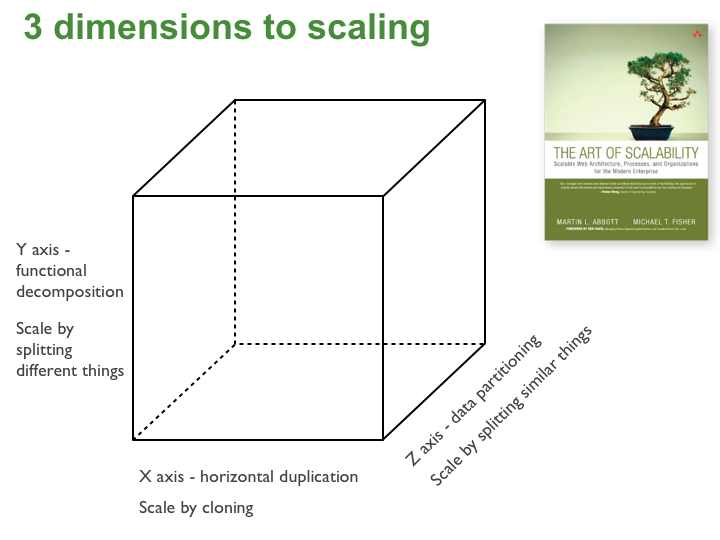
\includegraphics[width=\linewidth]{src/images/04-capitulo-4/scale_cube.jpg}
  \caption{El modelo de escalabilidad \eng{scale cube}}
  \label{fig:scale-cube}
\end{figure}

Como vimos en el Capítulo I, el diseño de la arquitectura del Integrador presentaba falencias que no permitían implementar redundancia ni escalar de manera eficiente, ya que para poder hacerlo, encontrábamos al menos dos inconvenientes: para lograr redundancia en el Integardor, era necesario replicar su instancia virtual y al mismo tiempo implementar alguna solución que redirija las peticiones a cualquiera de sus réplicas.  Además, debido a su diseño arquitectónico, sería necesario replicar cada \\gls{acro:api}, pero como se mencionó anteriormente, toda \gls{acro:api} se encontraba fuertemente acoplada a su aplicación, lo que forzaba replicar no solo la \gls{acro:api}, sino también la aplicación que generaba los datos.

Debido a esto, se planteó una nueva arquitectura de la nube de servicios de la {\unlp} que debe ser replicable y escalable. Para lograrlo, cada \gls{acro:api} correrá en una instancia virtual independiente, de manera tal que la misma pueda ser replicada tantas veces como sea necesario (\eng{X-axis scaling}). El punto de acceso a esta arquitectura replicada será un balanceador de carga que servirá tanto para balancear la carga como \eng{failover}, dando continuidad a los servicios en caso de que alguna de las instancias replicadas falle.

La característica fundamental de un balanceador de carga es ser capaz de distribuir las peticiones entrantes a un grupo de servidores (\eng{backends}) de acuerdo a un algoritmo de decisión y ponderación llamado \eng{scheduler}. Este algoritmo definirá cómo se toma la decisión, qué backend podría atender un requerimiento entrante, existiendo algunos simples (hacerlo de manera aleatoria o siguiendo un criterio ordenado por turnos como \eng{Round Robin}) y otros más sofisticados (que consideran otros factores como por ejemplo la carga de cada backend, su tiempo de respuesta promedio, el número de conexiones activas, la ubicación geográfica, etc.). En su funcionamiento básico el balanceador de carga redirige las peticiones a alguno de los backends, el cual luego contesta al balanceador, para que finalmente sea el balanceador el que entregue la respuesta al cliente sin que este último sepa de la existencia de esta compleja arquitectura. Esta estructura transparente al cliente evita accesos directos entre éste y los servidores que actúan como backend.

Como se mencionó anteriormente, el balanceador puede también ser usado como \eng{failover}, permitiendo que la falla de uno o más backends no afecten la disponibilidad del servicio. Los backends son monitoreados continuamente por el balanceador, cuando uno de estos falla, el balanceador deja de enviar tráfico al backend caído. Una vez que el backend vuelve a estar online, el balanceador detecta esta situación y comienza a enviarle tráfico nuevamente.

Según la RFC 7234\footnote{Este documento define las caches \gls{proto:http} y las cabeceras de control de cache permitidas en la versión \texttt{1.1} de ese protocolo\\\url{https://tools.ietf.org/html/rfc7234}}, una memoria cache almacena respuestas en pos de reducir el tiempo de respuesta y el consumo del ancho de banda. Asimismo, una memoria cache compartida es una cache que almacena respuestas para ser usadas por más de un cliente. Por lo tanto, delante del balanceador se implementará una caché compartida utilizando \gls{db:varnish}, la misma evitará los accesos al balanceador que puedan impactar de forma directa en alguna de las instancias replicadas de la {\cloud}, obteniendo mejores tiempos de respuesta así como tolerancia a fallos.

A modo de ejemplo, podemos pensar en una aplicación (\textit{cliente A}) que accede al servicio \url{/academic_units}. La petición es atendida por la API de referencia, donde el servicio devuelve todas la Unidades Académicas activas. Si más tarde otra aplicación (\textit{cliente B}), consulta la \gls{acro:api} por las Unidades Académicas, accediendo también al servicio \url{/academic_units} de la misma API, terminará obteniendo el mismo listado de Unidades Académicas. Como se puede apreciar, tenemos dos accesos a la API de referencia con idénticas respuestas, ambas procesadas por completo por uno o más backends. Esta situación puede evitarse con la inclusión de una cache compartida entre los diferentes clientes, logrando mejorar los tiempos de respuesta ya que la API recibirá únicamente un acceso, debiendo acceder y procesar los datos una única vez, ya que el resto de las peticiones serán obtenidas desde la cache compartida.


\subsubsection{Desacoplamiento}

Como se mencionó en \nameref{esb:introduccion}, uno de los 9 principios de diseño de \gls{acro:soa} es el bajo acoplamiento (\eng{loose coupling}), y quizás la forma más comunes de implementarlo es mediante un \gls{acro:esb}, quien se encargará de proveer interoperabilidad entre las diferentes plataformas. El acceso a la {\cloud} estará restringido a las direcciones IP de las aplicaciones (clientes) y al uso de un token, que se utilizará como autenticación. Este mecanismo de seguridad no será necesario desarrollarlo ya que se implementará en el \gls{acro:esb}.

Al mismo tiempo, en pos de trabajar en el desacoplamiento de las plataformas, se propone desarrollar una API dedicada a servir datos de referencia en la cual se implementarán los servicios necesarios que permitirán el acceso a los datos de referencia desde las distintas aplicaciones.

Para la solución planteada podemos observar las siguientes ventajas:

\begin{itemize}
  \item \textbf{Escalabilidad:} permite escalar horizontalmente (\eng{X-axis scaling}), es decir, en el hipotético caso que la API de referencia sea accedida por muchas aplicaciones, la misma podría replicarse en varias instancias, evitando la sobrecarga de cualquiera de ellas, al mismo tiempo que serviría como \eng{failover}.

  \item \textbf{Administración centralizada:} se centraliza la administración de los datos de referencia, evitando que la duplicidad se propague en cada aplicación que necesite utilizarlos.

  \item \textbf{Mantenimiento centralizado:} cuando hablamos de mantenimiento nos referimos a mejoras en la \gls{acro:api}, como por ejemplo, implementación de nuevos servicios, arreglo de errores, etc. Tener una API de referencia totalmente desacoplada de las aplicaciones que generan los datos permite actualizarla de forma más sencilla, evitando parar momentáneamente otras aplicaciones.

  \item \textbf{Agilización en el desarrollo:} otra de las ventajas que presenta este esquema, es la agilización en el desarrollo de nuevas aplicaciones. No será necesario desarrollar el módulo que administra los datos de referencia, los mismos se accederán vía servicios desde la API de referencia.  De esta manera, evitamos duplicar código fuente para implementar esta funcionalidad, al mismo tiempo que acortamos los tiempos de desarrollo.
\end{itemize}

En segunda instancia, se deberán escribir nuevamante todas las \glspl{acro:api} que se encuentran actualmente en producción. Para tal propósito, se utilizará el lenguaje de programación Ruby con el framework \nameref{soa:tecnologias:rails}, por los motivos que ya hemos expuesto en la \autoref{soa:tecnologias:para-servicios}. Esto dará origen a diferentes \eng{service components}, que antes se encontraban implementados dentro de cada aplicación y acopladas a la misma, y ahora estarán implementados en una nueva aplicación independiente y dedicada.  De esta manera desacoplamos la lógica de la aplicación, del acceso a los datos que se generan en la misma, permitiendo que esta solución escale horizontalmente de manera sencilla.

También se debe tener en cuenta que esta solución permite independizarse del lenguaje utilizado para el desarrollo de la aplicación: podemos desarrollar las aplicaciones en Ruby, PHP, JavaScript, Java o cualquier otro lenguaje, mientras que la \gls{acro:api} puede ser desarrollada utlizando el lenguaje Ruby. Esto genera una capa de servicios en gran parte independiente de las aplicaciones, cuya única dependencia radica en el modelo de datos de cada aplicación, ya que si se modifica el modelo de la aplicación se deberá modificar de manera acorde el acceso a los datos, es decir los servicios.


\subsubsection{Simplicidad}

Como se desarrolló en \autoref{microservicios}, las aplicaciones monolíticas consisten en componentes fuertemente acoplados, que son parte de una única unidad \eng{deployable}, resultando dificultosa la incorporación de cambios, \eng{testing} y \eng{deployment} de la aplicación.  El patrón de microservicios trata estas cuestiones, separando la aplicación en múltiples unidades \eng{deployables}, que pueden ser desarrolladas, testeadas y desplegadas de forma independientemente.

El hecho de dividir la aplicación en componentes pequeños y \eng{deployables} de manera independiente, facilita el desarrollo, \eng{testing} y puesta en producción, esto se debe a que el cambio se encuentra aislado a un \eng{service component}, permitiendo un mayor control.  Es por esto que hemos optado por seguir el patrón de arquitectura de microservicios para el diseño de la nube de servicios de la {\unlp}.

\subsubsection{Tolerancia a fallos}

Los sistemas distribuidos tienen potencialmente más fallos que los sistemas monolíticos, ya que en cada solicitud intervienen decenas (o cientos) de microservicios diferentes\cite[p.~48]{stin2015}. Es por esto que no resulta suficiente descomponer un sistema en componentes independientes; también hay que evitar que un fallo en uno de estos cause un fallo en cascada\cite[p.~4]{stin2015}, situación en que un error en una capa interna provoca un fallo en la capa más externa\cite[p.~65]{nygard2007}. Mike Nygard describe en su libro ``Release It!''\cite{nygard2007} varios patrones tolerantes a fallos, de los cuales el mas popular es el \eng{Circuit Breaker}.

\begin{figure}[H]
  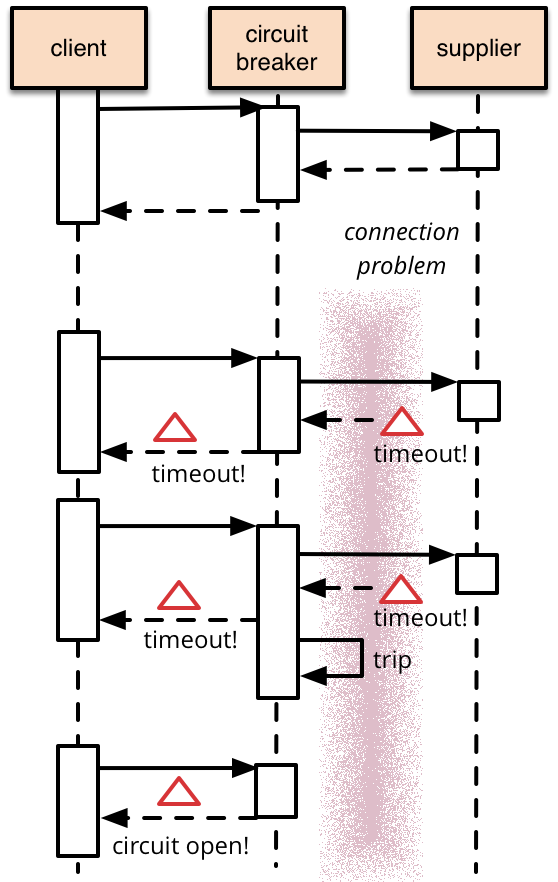
\includegraphics[width=\linewidth]{src/images/04-capitulo-4/circuit_breaker.png}
  \caption{Patrón de tolerancia a fallos \eng{Circuit Breaker}}
  \label{fig:circuit_breaker}
\end{figure}

Para implementar una infraestructura tolerante a fallos, los servicios deberán estar replicados en varias instancias virtuales y, como detallamos antes, delante de éstas se implementará un balanceador de carga, que permitirá distribuir las peticiones realizadas entre las instancias virtuales, al mismo tiempo, se deberá trabajar en limitar el alcance del fallo a nivel de servicio.  Cabe aclarar que el partón de microservicios, realiza un aporte importante en este orden, ya que al dividir la aplicación en \eng{service components} ailamos el problema, facilitando luego su eventual solución y \eng{deployment} en producción.

\subsubsection{Estandarización}

Según el diccionario de la Real Academia Española, un estándar es lo que sirve como tipo, modelo, norma, patrón o referencia. En nuestro caso, la estandarización es el proceso por el cual se establecen normas comunmente aceptadas que permiten la comunicación de diferentes aplicaciones.

Como mencionamos anteriormente, para cada aplicación que lo requiera se deberá implementar una \gls{acro:api} de acceso a los datos que ésta genere. Esta implementación se realizará basándose en la especificación \nameref{soa:tecnologias:json-api} detallada en la \autoref{soa:tecnologias:para-estructura}.

Esta estandarización facilitará el desarrollo de clientes que consuman información de los diferentes servicios de las \glspl{acro:api}, ya que definen reglas que especifican cómo se podrá acceder a los datos, cuál será su estructura de respuesta, e incluso asisten en lograr independencia del lenguaje con el que se escriban estos clientes, quienes simplemente deben respetar las especificaciones para implementar el acceso a los servicios.

\subsubsection{El uso del ESB}

Al ahondar en SOA e investigar diferentes tecnologías y patrones de arquitectura de software (\eng{layered arquitecture}, \eng{event-driven arquitecture}, \eng{microservices arquitecture}), vimos en el de patrón de microservicios una mejora sustancial, en simplicidad y alcance, que se adecuaba a nuestras necesidades, por eso reemplazamos el ESB por un \eng{API Gateway} que funciona como un ``message broker liviano''.

El \eng{API Gateway} implementado cumple con todas las tareas que realiza un \gls{acro:esb} (proveer conectividad, ruteo sencillo, manejo de seguridad, fiabilidad en los servicios, monitoreo y registro de actividades), menos en la transformación de datos y ruteo inteligente.  Esto resulta suficiente para el alcance de este trabajo, el cual nos permitirá lograr experiencia en la materia, para luego decidir, en caso de ser necesario, cambiar el ``message broker'' por un ESB robusto, como podría ser Mule ESB, Fuse ESB, WSO2 ESB, Synapse, entre otros.  Cabe aclarar, que este cambio no sería trascendental, ya que se trata de una capa de la arquitectura totalmente aislada que provee varios servicios (proveer conectividad, ruteo, manejo de seguridad, fiabilidad en los servicios, monitoreo y registro de actividades), los cuales se encuentran encapsulados o agrupados, lo que permitirá ser reemplazada sin afectar el resto de la arquitectura.  Esto es posible, debido que desde el inicio, basamos el diseño de la arquitectura en los principios que propone \gls{acro:soa}, logrando obtener los beneficios que este marco de diseño para la integración de aplicaciones propone.

\subsubsection{La arquitectura propuesta}

\todo{Ver si esto sirve, contar qué producto va en qué parte}

\begin{figure}
  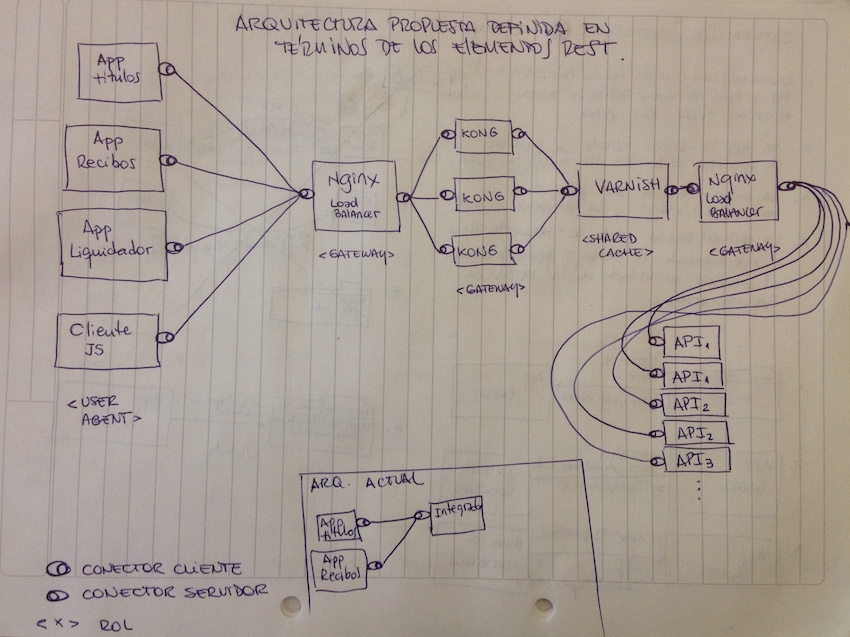
\includegraphics[width=\linewidth]{src/images/04-capitulo-4/nueva-arq-segun-rest.jpg}
  \caption{Visión \gls{acro:rest} de la nueva arquitectura propuesta}
  \label{fig:ejemplo-rest-nueva-arquitectura}
\end{figure}
